\documentclass[UTF8]{ctexart}
\usepackage{xcolor}
\definecolor{mygrn}{rgb}{0,0.6,0}
\definecolor{mygry}{rgb}{0.5,0.5,0.5}
\definecolor{mymau}{rgb}{0.58,0,0.82}

\usepackage{fancyvrb}
\usepackage{fancyhdr}
\pagestyle{fancy}
\fancyhf{}
\fancyhead[L]{\fangsong \leftmark}
\fancyfoot[R]{\thepage{}}

\usepackage{fontspec}
\setmonofont{Fira Mono}
\setsansfont{Consolas}
\setmainfont{Times New Roman}
\newfontfamily\fira{Fira Mono}
\newfontfamily\consolas{Consolas}
% if no found some fonts, comment it

\usepackage[text={148mm,220mm},centering,includehead,vmarginratio=1:1]{geometry}                    % 设置版面
\setlength{\headwidth}{\textwidth}                          % 设置页眉宽度
\setlength{\headheight}{14pt}                               % 设置页眉高度

\title{\vspace{10mm}\heiti\huge 地空系并行集群使用说明\vspace{30mm}}
\author{\LARGE\textsc{Tche LIU}\thanks{tcheliu@mail.ustc.edu.cn},~
\textsc{Gongheng ZHANG}\thanks{11749276@mail.sustc.edu.cn}
\vspace{10mm}}
\date{\today}

\usepackage{titlesec}
\titleformat{\section}{\Large\bf\flushleft}{\chinese{section}、\kern -1em}{1em}{}%[\vspace{2pt}{\titlerule*[3pt]{\textperiodcentered}}]

\usepackage{enumerate}                                      % 排序列表宏包 for enumerate 环境
\usepackage{amsmath}										% 公式宏包 for gather 环境
\usepackage{nicefrac}										% 斜分数宏包 for \nicefrac 斜分数命令
\usepackage{amssymb}										% 数学字符宏包 for 黑色方块和三角

\usepackage[colorlinks,linkcolor=blue,anchorcolor=yellow,citecolor=green]{hyperref}      % hyperreference package
\usepackage{graphicx}                                       % 绘图宏包 for \includegrahpics 命令
\usepackage{booktabs}                                       % for \toprule, \midrule and \bottomrule

\usepackage{listings}
\lstdefinestyle{bashsty}{ %
  backgroundcolor=\color{white},                 % choose the background color; you must add \usepackage{color} or \usepackage{xcolor}
  basicstyle=\ttfamily\scriptsize,               % the size of the fonts that are used for the code
% basicstyle=\consolas\scriptsize,               % the size of the fonts that are used for the code
  breakatwhitespace=false,                       % sets if automatic breaks should only happen at whitespace
  breaklines=true,                               % sets automatic line breaking
  captionpos=b,                                  % sets the caption-position to bottom
  commentstyle=\color{mygrn},                    % comment style
  deletekeywords={},                             % if you want to delete keywords from the given language
  escapeinside={\%*}{*)},                        % if you want to add LaTeX within your code
  extendedchars=true,                            % lets you use non-ASCII characters; for 8-bits encodings only, does not work with UTF-8
  firstnumber=1,                                 % Line numbers begin at line 1
  frame=single,	                                 % adds a frame around the code
  keepspaces=true,                               % keeps spaces in text, useful for keeping indentation of code (possibly needs columns=flexible)
  keywordstyle=[1]\color{blue},                  % keyword style
  keywordstyle=[2]\color{red},
  language=bash,                                 % the language of the code
  morekeywords=[1]{...},                         % Add any functions no included by default here separated by commas
  morekeywords=[2]{...},
  otherkeywords={...},                           % if you want to add more keywords to the set
  numbers=left,                                  % where to put the line-numbers; possible values are (none, left, right)
  numbersep=5pt,                                 % how far the line-numbers are from the code
  numberstyle=\tiny\color{mygry},                % the style that is used for the line-numbers
  rulecolor=\color{black},                       % if not set, the frame-color may be changed on line-breaks within not-black text (e.g. comments (green here))
  showspaces=false,                              % show spaces everywhere adding particular underscores; it overrides 'showstringspaces'
  showstringspaces=false,                        % underline spaces within strings only
  showtabs=false,                                % show tabs within strings adding particular underscores
  stepnumber=5,                                  % the step between two line-numbers. If it's 1, each line will be numbered
  stringstyle=\color{mymau},                     % string literal style
  tabsize=2,	                                 % sets default tabsize to 2 spaces
}

\newcommand{\mynote}[1]{\colorbox{gray!35}{#1}}
\newcommand{\mynnote}[1]{\colorbox{gray!15}{\color{blue}#1}}
\newcommand{\insertbash}[2]{\begin{itemize}\item[]\lstinputlisting[caption=#2,label=#1,style=bashsty]{#1}\end{itemize}}

\begin{document}

\maketitle
\centerline{Version: 0.2}
\newpage
\tableofcontents
\newpage

\section{注意事项}
\begin{enumerate}[\hspace{15mm}(1)]
  \item 严禁在任何节点直接运行并行程序,
    所有多核任务必需经由作业系统提交运行;
  \item 提交作业时务必注意节点的内存限制,
    切勿提交超负荷任务;
  \item 提交作业时烦请注意队列的提交限制,
    以防提交无效作业;
  \item 用户 HOME 目录所在磁盘 share 为全节点共享,
    该磁盘所有用户的用户配额为 1TB,
    当用户的总数据量超过该限制时,
    该用户将无法创建新文件;
  \item 请注意及时备份集群上的重要数据,
    本集群不保证用户数据的安全性;
  \item 为规范使用,仅允许用户在其作业运行期间,
    ssh 登录到相应的计算节点查看作业运行情况;
  \item 本集群虽安装有 matlab 等绘图软件,
    但不推荐在集群上直接成图,
    建议将数据拷贝到本地机器上,
    再利用本地机器作图。
\end{enumerate}

\section{LSF 作业调度系统}
\subsection{集群队列设置}
\begin{table}[h]
  \centering
  \caption{集群队列设置}
  \begin{tabular*}{400pt}{@{\extracolsep{\fill}}ccccccc}
    \toprule
    节点      & 队列  & 核数 & 内存  & 作业最长运行时间 & 优先级 & 交互式提交 \\
    \midrule
    mn01      & dataq & 20   & 62.1G & -      & 33 & 禁止 \\
    c001-c028 & short & 28   & 125G  & 12:00  & 40 & 禁止 \\
    c001-c028 & long  & 28   & 125G  & 无限制 & 30 & 允许 \\
    c029-c042 & large & 24   & 188G  & 48:00  & 30 & 禁止 \\
    s001-s002 & smp   & 72   & 508G  & 24:00  & 20 & 禁止 \\
    \bottomrule
  \end{tabular*}
\end{table}

注意,\mynote{mn01} 为主节点,
禁止在此节点运行作业。

在设置程序使用每节点核数时,
尽量设置为节点总核数的整除数。

\subsection{查询系统运行情况}
通过命令 \mynnote{lnodes},
可查看系统各节点连接情况。

通过命令 \mynnote{lshosts},
可查看系统各节点硬件配置情况。

通过命令 \mynnote{lsload},
可查看系统各节点当前负载。

通过命令 \mynnote{lsmon},
可动态查看系统各节点当前负载。

通过命令 \mynnote{bhosts},
可查看系统各节点作业运行情况。

通过命令 \mynnote{bqueues},
可查看系统中各队列作业运行情况。

通过命令 \mynnote{busers all},
可按用户查看所有用户的作业运行整体情况。

通过命令 \mynnote{bjobs -u all},
可按作业查看所有用户的作业运行详细情况。

通过命令 \mynnote{bhist -t -T <起始时刻,终止时刻>},
可按时间顺序查看某一时间段内作业系统的调度历史。

\subsection{LSF 作业提交}
\subsubsection{作业提交脚本的书写}
\insertbash{material/lsf.sh}{LSF 作业提交脚本示例}

在书写作业提交脚本时,LSF 作业系统主要的解析制导指令有:
\begin{enumerate}[\hspace{15mm}(1)]
  \item \mynnote{\#BSUB -J <作业名>}:指定作业名;
  \item \mynnote{\#BSUB -q <队列名>}:指定排队队列,
    此项不指定则调用默认队列;
  \item \mynnote{\#BSUB -n <申请总核数>}:指定总核数,
    此项不指定则总核数默认为 1;
  \item \mynnote{\#BSUB -R "<描述信息>"}:指定资源限制,
    这里的{\em 描述信息}可以为:\newline
    \mynnote{span[ptile=<每个节点的核数>]} 指定每节点使用核数、\newline
    \mynnote{span[phost=<节点数>]} 指定使用节点数、\newline
    \mynnote{rusage[mem=<每个节点的内存限制>]} 指定每核可用内存最低限制、\newline
    等内容;
  \item \mynnote{\#BSUB -W <挂钟时间>}:指定作业最长运行时间,
    时间格式为 hh:mm;
  \item \mynnote{\#BSUB -o <标准输出文件名>}:指定标准输出文件;
  \item \mynnote{\#BSUB -e <错误输出文件名>}:指定标准错误输出文件;
\end{enumerate}

另外注意,在编译程序过程中若使用了特别版本的编译器或运行库,
需在作业提交脚本中通过命令 \mynnote{module load <模块名>}
加载这些编译器或运行库环境模块。

\subsubsection{依赖作业提交}
通过在作业提交脚本头部中加入 \mynnote{\#BSUB -W "<复合作业状态>(<作业号>)"} 的内容,
可以实现相互依赖的多个作业任务的提交。
当指定作业达到指定状态时,
当前作业才会被派发。

这里的{\em 复合作业状态}可以设置为:
\begin{enumerate}[\hspace{15mm}(1)]
  \item started: 指定作业开始运行或已完成,
    即基本作业状态除 PEND 和 PSUSP 之外的其他状态;
  \item done: 基本作业状态 DONE;
  \item ended: 基本作业状态 EXIT 或 DONE;
  \item exit: 基本作业状态 EXIT,
    可通过 \mynnote{(<作业号>,[操作符] <退出码>)} 指定特殊的退出码,
    这里的{\em 操作符}可以设为 >、>=、<、<=、== 或 !=;
  \item started: 基本作业状态 DONE、EXIT、USUSP、SSUSP 或 RUN。
\end{enumerate}
基本作业状态参见下文内容。

通过命令 \mynnote{bjdepinfo <作业号>},
可查看已提交作业的依赖关系。

\subsection{LSF 作业管理}
\subsubsection{LSF 作业状态}
LSF 调度系统的基本作业状态有:
\begin{enumerate}[\hspace{15mm}(1)]
  \item PEND: 在系统中排队,等待派发;
  \item RUN: 已经被派发,在运行中;
  \item DONE: 正常运行完毕,程序退出码为 0;
  \item PSUSP: 被用户自己或管理员在派发前挂起;
  \item USUSP: 被用户自己或管理员在派发后挂起;
  \item SSUSP: 被 LSF 系统在派发后挂起;
  \item EXIT: 被异常终止,或程序退出码非 0。
\end{enumerate}

被用户自己或管理员挂起的作业不会被系统自动派发;
被系统挂起的作业待满足运行条件后系统会自动派发。

作业被系统挂起的原因有:
该作业依赖于其他待完成作业、
该作业在队列中的优先级较低、
没有足够的计算资源等。

\subsubsection{LSF 作业调度}
\begin{figure}[h]
  \centering
  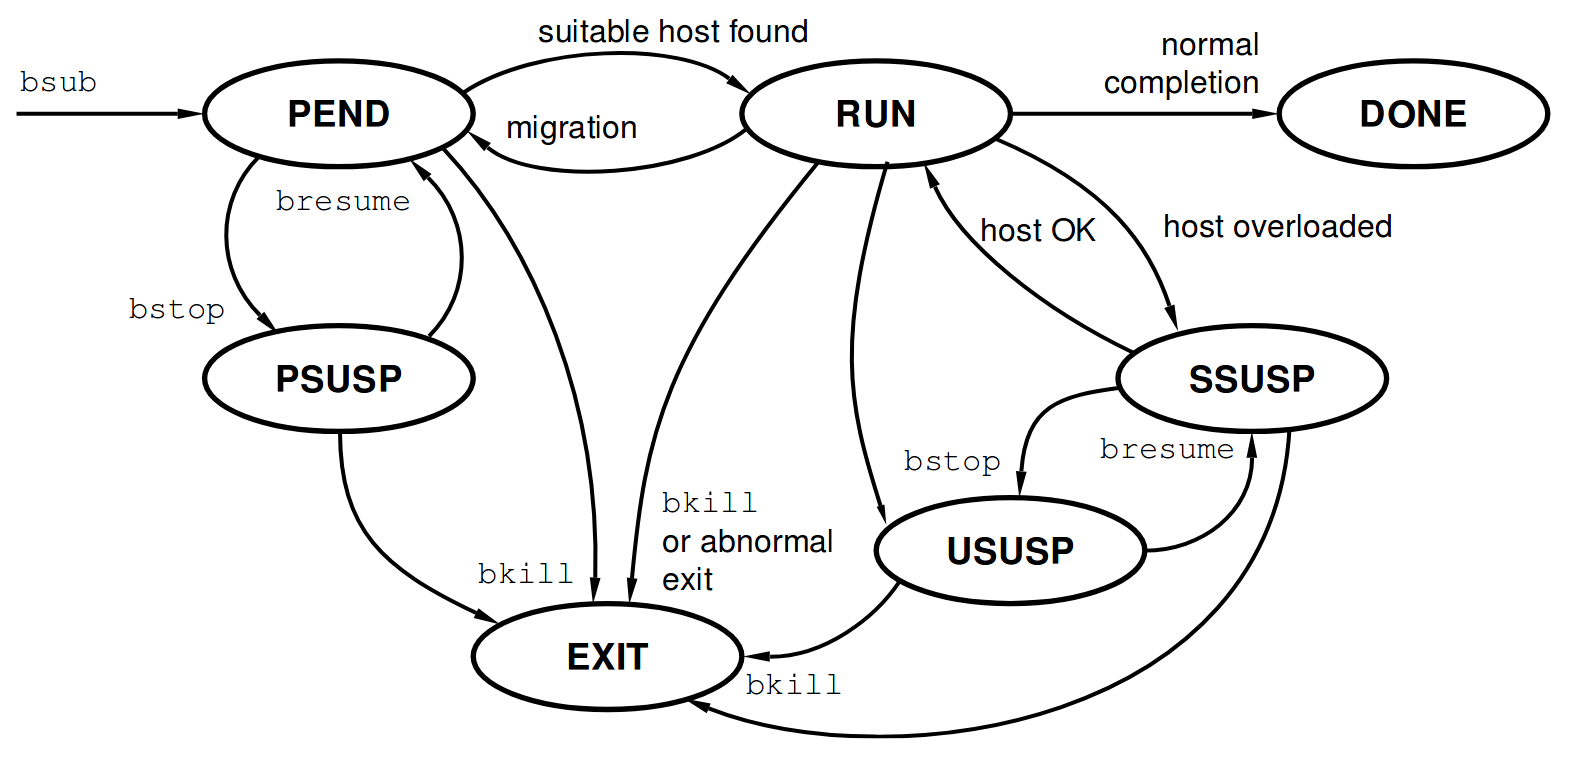
\includegraphics[width=140mm]{material/bjobstate.png}
  \caption{LSF 基本作业状态}
\end{figure}

参照前述示例正确书写作业提交脚本 job.lsf 后,
即可通过命令 \mynnote{bsub < job.lsf} 提交作业。
正确提交作业后,该命令会返回系统分配的作业号。
区别于 PBS 作业系统,注意{\color{red}\em 这里的“<”是必需的}。

作业提交后,通过命令 \mynnote{bjobs -l <作业号>},
可以查看作业状态。

作业提交后,通过命令 \mynnote{bstop <作业号>},
用户可以将自己的正在排队(PEND 状态)的作业挂起(PSUSP 状态);
此时,可以通过命令 \mynnote{bresume <作业号>},
将挂起(PSUSP 状态)的作业重新参与系统排队(PEND 状态),
等待系统派发。

作业开始运行后,同样可以通过 bstop 命令,
用户可以将自己的正在运行(RUN 状态)的作业挂起(USUSP 状态);
同样地,通过 bresume 命令,
再次将挂起(USUSP 状态)的作业重新参与系统排队(SSUSP 状态),
等待系统派发。

通过命令 \mynnote{bkill <作业号>},
用户可以将自己待运行或正在运行的作业取消(EXIT 状态)。

通过命令 \mynnote{bkill -s <系统消息代码> <作业号>},
用户可以向自己的正在运行的作业发送系统消息。

通过命令 \mynnote{bhist -l <作业号>},
用户可以查看指定作业的系统调度历史。

通过命令 \mynnote{bpeek <作业号>},
用户可以查看自己的未完成作业的标准输出和错误输出。

在作业完成后,LSF 系统会保留作业记录 5 分钟,
此时,还可以通过作业号查看作业的运行记录。

\subsection{参考阅读}
\href{http://hpc.sustech.edu.cn/ref/lsf_users_guide_v10.1.pdf}{LSF 用户手册}:
http://hpc.sustech.edu.cn/ref/lsf\_users\_guide\_v10.1.pdf

\href{http://hpc.sustech.edu.cn/ref/TaiYi_User_Manual_v0.1.pdf}{太乙用户手册}:
http://hpc.sustech.edu.cn/ref/TaiYi\_User\_Manual\_v0.1.pdf

\href{https://www.ibm.com/support/knowledgecenter/en/SSWRJV_10.1.0/lsf_welcome/lsf_welcome.html}{IBM Spectrum LSF V10.1 documentation}:
https://www.ibm.com/support/\newline
knowledgecenter/en/SSWRJV\_10.1.0/lsf\_welcome/lsf\_welcome.html

\href{https://ls11-www.cs.tu-dortmund.de/people/hermes/manuals/LSF/users.pdf}{LSF Batch User's Guide}:
https://ls11-www.cs.tu-dortmund.de/people/hermes/manuals/\newline
LSF/users.pdf

\section{Module Environment 的使用}
\subsection{系统软件环境}
\subsubsection{系统软件安装目录}
系统软件的安装目录主要有:\newline
/share/apps: 安装了 python 和 java 的解释器;\newline
/share/base: 安装了大部分的运行库和一部分工具;\newline
/share/intel: 安装了 intel 编译器及附带工具;\newline
/share/tools: 安装了一些工具。

\subsubsection{编译器及解释器}
系统安装了多个版本的 C 和 Fortran 语言编译器:\newline
系统默认的 gcc/4.8.5 (系统标准安装目录)、\newline
gcc/8.2.0 (/share/base/gcc/8.2.0 目录)、\newline
intel/2017.8 (/share/intel/2017u8 目录)、\newline
intel/2018.3 (/share/intel/2018u3 目录)、\newline
intel/2018.4 (/share/intel/2018u4 目录)。
\bigskip

系统安装了多个版本的 Python 语言解释器:\newline
python/2.7.15 (/share/apps/python/2.7.15 目录)、\newline
python/3.7.0 (/share/apps/python/3.7.0 目录)、\newline
python/anaconda2/5.2.0 (/share/apps/anaconda2/5.2.0 目录)、\newline
python/anaconda3/5.2.0 (/share/apps/anaconda3/5.2.0 目录)、\newline
python/intelpython2/2018.3.039 (/share/apps/ipython/2018.3.039/intelpython2 目录)、\newline
python/intelpython2/2019.9.047 (/share/apps/ipython/2019.9.047/intelpython2 目录)、\newline
python/intelpython3/2018.3.039 (/share/apps/ipython/2018.3.039/intelpython3 目录)、\newline
python/intelpython3/2019.9.047 (/share/apps/ipython/2019.9.047/intelpython3 目录)。
\bigskip

系统安装了一个版本的 matlab 语言解释器:\newline
matlab/R2018b (/share/apps/matlab/Matlab 目录)。
\bigskip

系统安装了一个版本的 go 语言编译器:\newline
go/1.11.1 (/share/base/go/1.11.1 目录)。
\bigskip

系统安装了两个版本的 java 语言解释器:\newline
java/1.8.0\_181 (/share/apps/java/1.8.0\_181 目录)、\newline
java/10.0.2 (/share/apps/java/10.0.2 目录)。

\subsubsection{运行库}
系统安装的运行库大部分都同时有 gcc/4.8.5 和 intel/2018.4 两个编译器的版本。
\bigskip

系统安装的 MPI 并行库有:\newline
mpi/intel (在各自对应版本的 intel 编译器安装目录下)、\newline
mpi/mpich (/share/base/mpich 目录)、\newline
mpi/openmpi (系统标准安装目录或 /share/base/openmpi 目录)。
\bigskip

系统安装的其他第三方运行时函数库主要有:\newline
zlib (/share/base/zlib 目录)、\newline
fftw (/share/base/fftw 目录)、\newline
hdf5 (/share/base/hdf5 目录)、\newline
netcdf-c (/share/base/netcdf-c 目录)、\newline
netcdf-fortran (/share/base/netcdf-fortran 目录)、\newline
netcdf-cxx (/share/base/netcdf-cxx 目录)。

\subsubsection{工具}
系统安装的软件编译安装工具有:\newline
系统默认的 make/3.82 (系统标准安装目录)、\newline
make/4.2 (/share/tools/make/4.2 目录)、\newline
系统默认的 cmake/2.8.12.2 (系统标准安装目录)、\newline
cmake/3.12.2 (/share/base/cmake/3.12.2 目录)、\newline
meson/0.50.0 (/share/tools/meson/0.50.0 目录)、\newline
ninja/1.9.0 (/share/tools/ninja/1.9.0 目录)。
\bigskip

系统安装的绘图工具有:\newline
GMT/4.5.18 (/share/tools/GMT/4.5.18 目录)、\newline
GMT/5.4.5 (/share/tools/GMT/5.4.5 目录)。
\bigskip

系统安装的其他辅助工具有:\newline
系统默认的 git/1.8.3.1 (系统标准安装目录)、\newline
git/2.18.0 (/share/base/git/2.18 目录)、\newline
htop/2.2.0 (/share/base/htop/2.2.0 目录)、\newline
parallel/20180922 (即 GNU Parallel,/share/base/parallel 目录)。

\subsection{module 的使用}
当在 Linux 下存在多个版本的同一个编译器或运行库时,
如果每次编译都写上绝对路径就很麻烦,
使用 module-environment (以下简称 module )来{\em 管理环境变量}则相比方便很多。

例如,在我们服务器中安装了多个版本的 intel 编译器,包括:
intel/2017.8、intel/2018.3 和 intel/2018.4。
在调用 intel/2017.8 时,
一般先要修改 PATH 和 LD\_LIBRARY\_PATH 等系统环境变量。
此时若要改为调用 intel/2018.4,
又要再次修改这些环境变量,
容易造成混乱。
使用 module 则可以通过方便地 modulefile 进行系统环境变量的配置。

\subsubsection{搜索路径 MODULEPATH}
module 的搜索路径由系统环境变量 MODULEPATH 定义,
在 MODULEPATH 包含的路径下的 modulefile 文件,
可以自动被 module 识别。
非 root 用户可以通过修改 MODULEPATH 加入自己的 modulefile 目录,
从而实现通过 module 来管理自己在 home 目录下单独安装的软件。

\subsubsection{自定义 modulefile 文件}
在自定义 modulefile  文件时需注意,
文件必需以 \mynote{\#\%Module} 开头,
这样才会被 module 识别为 modulefile 文件。

常用的 modulefile 命令有:
\begin{enumerate}[\hspace{15mm}(1)]
  \item \mynote{module-whatis "模块描述"}:添加对该 module 的描述信息;
  \item \mynote{conflict <模块名>}:如果这里指定的模块已被加载,
    当前定义的模块将不会被加载;
  \item \mynote{set <变量名> <值>}:设置变量,
    这里定义的变量仅在该 modulefile 文件中生效;
  \item \mynote{setenv <系统环境变量名> <值>}:设置系统环境变量,
    将系统环境变量重置。这里定义的变量将在加载该模块后对整个系统生效;
  \item \mynote{prepend-path <系统环境变量名> <新添值>}:设置系统环境变量,
    在原变量值{\em 前}添加新的内容。
\end{enumerate}

\insertbash{material/module.sh}{modulefile 文件书写示例}

更多示例参见服务器上 /share/base/modulefiles/ 目录。

\subsubsection{module 模块命令}
module 模块命令有:
\begin{enumerate}[\hspace{15mm}(1)]
  \item \mynnote{module avil [模块名]}:查看系统可用的模块;
  \item \mynnote{module list}:查看已经加载的模块;
  \item \mynnote{module whatis [模块名]}:查看模块描述信息;
  \item \mynnote{module load <模块名>}:加载指定模块;
  \item \mynnote{module unload <模块名>}:卸载指定模块;
  \item \mynnote{module purge}:卸载所有已加载的模块。
\end{enumerate}

例如,我们要调用 intel/2017.8 来编译程序,
可先由命令 \mynote{module load intel/2017.8} 加载该软件模块环境后,
即可直接通过命令 icc/ifort 调用该模块的编译器来编译程序。

此时,若想换用 intel/2018.4 模块,
可先由命令 \mynote{module unload intel/2017.8} 卸载 intel/2017.8 模块后,
再由命令 \mynote{module load intel/2018.4} 加载 intel/2018.4 模拟后即可。

另外,在调用 mpi/intel 模块时请注意,
mpicc/mpif90 实际最终调用的还是 GNU 编译器;
{\color{red}\em 若想调用 intel 编译器,请使用 mpiicc/mpiifort 命令},
此时还需额外加载相应的 intel 编译器模块。

\subsubsection{参考阅读}
\href{https://modules.readthedocs.io/en/stable/module.html}{module 命令手册}:
https://modules.readthedocs.io/en/stable/module.html

\href{https://modules.readthedocs.io/en/stable/modulefile.html}{modulefile 配置手册}:
https://modules.readthedocs.io/en/stable/modulefile.html

\href{https://blog.csdn.net/jslove1997/article/details/80338370}{module 简单使用}:
https://blog.csdn.net/jslove1997/article/details/80338370

\end{document}
